\section{Privacy in machine learning}

\only<article>{ Consider a researcher wishing to collect data for a
  statistical analysis. As long as the analysis is eventually
  published,\footnote{If somebody knows that the analysis is being
    conducted, however, they could still learn something private from
    the fact that the analysis has /emph{not} been published.} this
  creates two types of possible privacy violations. The first is
  direct exposure of sensitive data through publication of the
  analysis, if for example the study is about something such as drug
  use. The second is through publication of ``anonymised'' versions of
  the dataset, which create opportunities for linkage attacks.}

\begin{figure}[h]
  \begin{tikzpicture}
    \node[label=left:$x$] at (0,0) (data) {
\includegraphics[width=0.3\columnwidth]{../figures/medical}};

    \node[label=$x_1$] at (-2,3)(patient1) {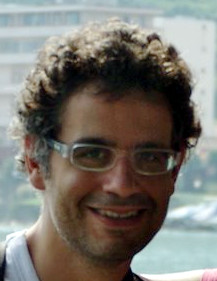
\includegraphics[width=0.1\columnwidth]{../figures/me-recent}};
    \uncover<3->{
      \node[label=$x_2$] at (2,3) (patient2) {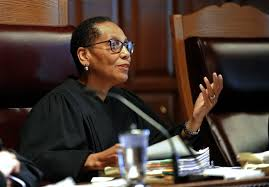
\includegraphics[width=0.2\columnwidth]{../figures/judge}};
    }
    \uncover<4->{
      \node[label=$a$] at (4,0)   (statistics) {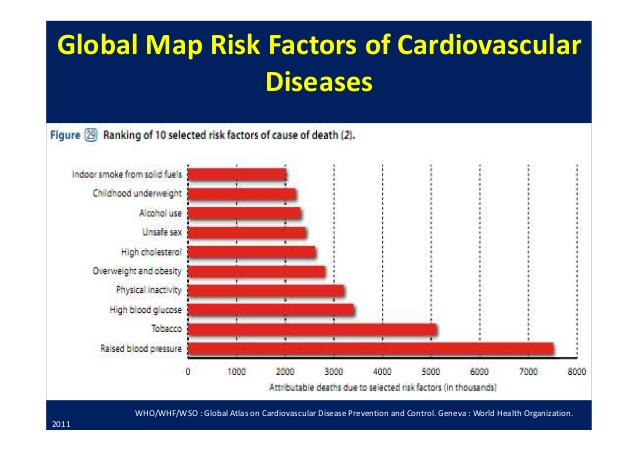
\includegraphics[width=0.3\columnwidth]{../figures/coronary-disease}};
    }
    \uncover<2->{
      \draw[->] (patient1) -- (data);
    }
    \uncover<3->{
      \draw[->] (patient2) -- (data);
    }
    \uncover<4->{
      \draw[->] (data) -- node[above]{$\pol$} (statistics);
    }
    \uncover<5->{
      \draw[line width=5, red, ->] (statistics) -- (patient2);
    }
  \end{tikzpicture}
  \caption{If two people contribute their data $x = (x_1, x_2)$ to a medical database, and an algorithm $\pol$ computes some public output $a$ from $x$, then it should be hard infer anything about the data from the public output.}
\end{figure}
\section{The random response mechanism.}
\begin{frame}
  \frametitle{Asking about drug use}

  \only<article>{
    Let's say you need to perform a statistical analysis of the drug-use habits of athletes. Obviously, even if you promise the athlete not to reveal their information, you still might not convince them. Yet, you'd like them to be truthful. The trick is to allow them to randomly change their answers, so that you can't be \emph{sure} if they take drugs, no matter what they answer.
  }

  \begin{example}[Randomising responses about drug use]
    \begin{enumerate}
    \item Flip a coin.
    \item If it comes heads, respond \texttt{Yes}.
    \item Otherwise, respond truthfully.
    \end{enumerate}
  \end{example}

  If the rate of positive responses is $p$, everybody follows the protocol, and the coin is fair, what is the true rate $q$ of drug use?
  \only<presentation>{
    \uncover<2>{
      \[
      p = 1/2 + q/2 \Rightarrow q = 1/2
      \]
    }
  }
  \only<article>{The problem with this approach, of course, is that we are effectively throwing away half of our data. In particular, if we repeated the experiment with a coin that came heads at a rate $\epsilon$, then our error bounds would scale as $O(1/\sqrt{\epsilon n})$ for $n$ data points.}
\end{frame}

\begin{frame}
  \frametitle{The randomised response mechanism}
  \only<article>{The above idea can be generalised. Consider we have data $x_1, \ldots, x_n$ from $n$ users and we transform it randomly to $y_1, \ldots, y_n$ using the following mapping.}
  \begin{definition}[Randomised response]
    The $i$-th user, whose data is $x_i \in \CX$ , responds with $y_i \in \CX$ with probability
    \[
    \Pr(y_i = j \mid x_i = k) = p_{kj},
    \]
    where $p_{kk} > p_{kj} \forall J$.
  \end{definition}
  \only<article>{This mechanism satisfies so-called $\epsilon$-differential privacy.}
\end{frame}

\begin{frame}
  \frametitle{The statistical privacy framework}
  
  \begin{tikzpicture}
    \node at (0,0) (x) {Data};
    \node at (4,2) (mech) {Algorithm};
    \node at (4,0) (private) {Output};
    \node at (8,0) (access) {Observer};
    \draw [->] (x) -- (private);
    \draw [->] (mech) --(private);
    \draw [<->] (private) -- (access);
  \end{tikzpicture}

  \only<article>{
    Consider a scenario where $n$ persons give their data $x_1, \ldots, x_n$ to an analyst. This analyst then performs some calculation $f(x)$ on the data and published the result. The following properties are desirable from a general standpoint.

    \paragraph{Anonymity.} Individual participation in the study remains a secret. From the release of the calculations results, nobody can significantly increase their probability of identifying an individual in the database.

    \paragraph{Secrecy.} The data of individuals is not revealed. The release does not significantly increase the probability of inferring individual's information $x_i$.

    \paragraph{Side-information.} Even if an adversary has arbitrary side-information, he cannot use that to amplify the amount of knowledge he would have obtained from the release.

    \paragraph{Utility.} The released result has, with high probability, only a small error relative to a calculation that does not attempt to safeguard privacy.
  }
  \only<presentation>{
    \begin{itemize}
    \item Anonymity: Individual participation remains hidden.
    \item Secrecy: Individual data $x_i$ is not revealed.
    \item Side-information: Linkage attacks are not possible.
    \item Utility: The calculation remains useful.
    \end{itemize}
  }
\end{frame}

\begin{frame}
  \frametitle{Differential privacy.}

  \only<article>{Now let us take a look at a way to characterise the  the inherent privacy properties of algorithms. This is called differential privacy, and it can be seen as a bound on the information an adversary with arbitrary power or side-information could extract from a computation.}

  \begin{definition}[$\epsilon$-Differential Privacy]
    A stochastic algorithm $\pol : \CX \to \CY$, where $\CX$ is endowed with a neighbourhood relation $N$, is said to be $\epsilon$-differentially private if
    \begin{equation}
      \label{eq:epsilon-dp}
      \pol(y \mid x) \leq \pol(y \mid x'), \qquad \forall x N x'.
    \end{equation}
  \end{definition}
  
  \only<article>{Typically, algorithms are applied to datasets $x = (x_1, \ldots, x_n)$ composed of the data of $n$ individuals. Thus, all privacy guarantees relate to the data contributed by these individuals. 

    In this context, two datasets are usually called neighbouring if $x = (x_1, \ldots, x_{i-1}, x_i, x_{i+1} x_n)$ and 
    $x' = (x_1, \ldots, x_{i-1}, x_{i+1} x_n)$, i.e. if one dataset is missing an element.
    
    A slightly weaker definition of neighbourhood is to say that $x N x'$ if $x' = (x_1, \ldots, x_{i-1}, x'_i, x_{i+1} x_n)$, i.e. if one dataset has an altered element.

  }

  \begin{remark}
    Any differentially private algorithm must be stochastic.
  \end{remark}
  \only<article>{
    To prove that this is necessary, consider the example of counting how many people take drugs in a competition. If the adversary only doesn't know whether you in particular take drugs, but knows whether everybody else takes drugs, it's trivial to discover your own drug habits by looking at the total. This is because in this case, $f(x) = \sum_i x_i$ and the adversary knows $x_i$ for all $i \neq j$. Then, by observing $f(x)$, he can recover $x_j = f(x) - \sum_{i \neq j} x_i$. Consequently, it is not possible to protect against adversaries with arbitrary side information without stochasticity.}
  \begin{remark}
    The randomised response mechanism is $\epsilon$-DP.
  \end{remark}
\end{frame}

\section{Statistical inference}
\only<article>{Statistical inference is the problem estimating quantities from data. Many machine learning problems lie within the statistical inference framework. While there are many paradigms within this framework, one typically tries to calculate probability distributions of some random variables from data. These are usually expressed in terms of parametrised distributions. In the Bayesian setting in particular, the goal is to quantify our uncertainty about these unknown parameters in terms of another probability distribution.}
\begin{frame}
  \frametitle{Bayesian inference} \only<article>{ Bayesian statistical
    inference is the problem of inferring distributions (of
    parameters) from data. Typically, given some prior distribution
    $\bel(\param)$ on parameters $\param \in \Param$, such that for
    every possible parameter value the probability $P_\param(x)$ is
    well defined for any $x \in \CX$, we wish to infer a posterior
    distribution from any given data $x$.}
  \begin{definition}[Posterior distribution]
    \only<article>{Given a prior $\bel$ on the parameter set $\Param$
      and a family $\{P_\param\}$ of distributions on $\CX$, the
      posterior distribution of parameter $\param$ for any data
      $x \in \CX$ is}
    \begin{equation}
      \bel(\param \mid x) \defn \frac{P_\param(x) \bel(\param)}{\sum_{\param' \in \Param}
        P_{\param'}(x) \bel(\param')}.
      \label{eq:posterior}
    \end{equation}
  \end{definition}
  \only<article>{But ...}
\end{frame}



\begin{frame}
  \frametitle{The Laplace mechanism.}
  \only<article>{
    A simple method to obtain a differentially private algorithm from a deterministic function $f : \CX \to \Reals$, is to use additive noise. 
  }
  \begin{definition}[The Laplace mechanism]
    For any function $f : \CX \to \Reals$, 
    \begin{equation}
      \label{eq:laplace-mechanism}
      \pol(a \mid x) = \Laplace(f(x), \lambda).
    \end{equation}
  \end{definition}
  \only<article>{Here, $\Laplace(\mu, \lambda)$ is the density $f(x) = \frac{\lambda}{2} \exp(-\lambda |x - \mu|)$}.



\end{frame}



%%% Local Variables:
%%% mode: latex
%%% TeX-engine: xetex
%%% TeX-master: "notes"
%%% End:

